\documentclass[border=5pt]{standalone}
\usepackage[T1]{fontenc}
\usepackage{lmodern}
\usepackage{pgfplots}
\usepgfplotslibrary{groupplots}
\pgfplotsset{compat=1.18}
\begin{document}\sffamily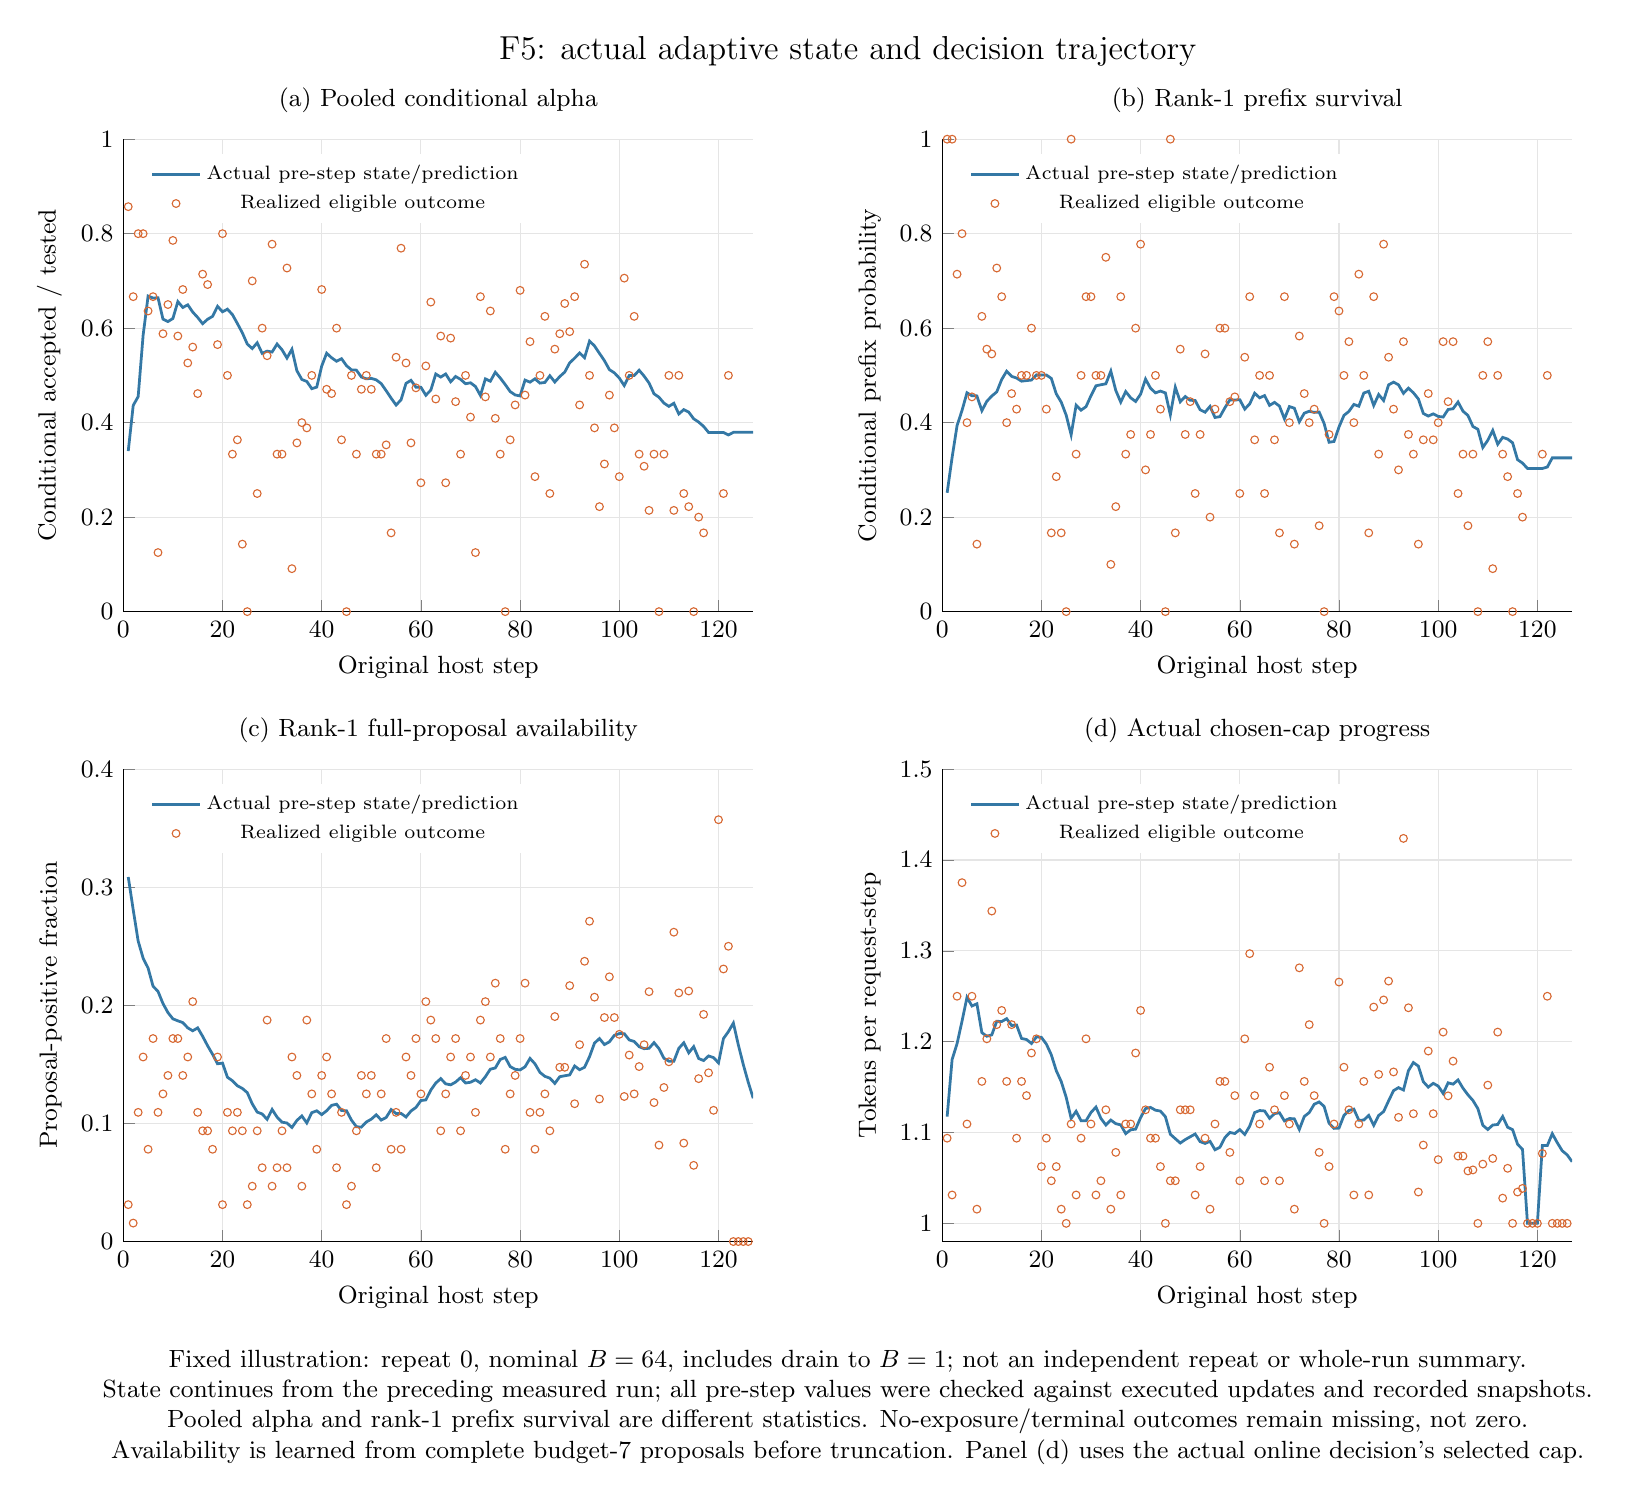
\begin{tikzpicture}
\definecolor{cal}{HTML}{3478A5}\definecolor{test}{HTML}{D76832}\definecolor{profile}{HTML}{3B8A5A}
\begin{groupplot}[group style={group size=2 by 2,horizontal sep=2.4cm,vertical sep=2.0cm},width=8.0cm,height=6.0cm,scale only axis,axis lines*=left,grid=major,grid style={gray!20},tick label style={font=\small},label style={font=\small},title style={font=\small},legend style={font=\scriptsize,draw=none},unbounded coords=jump]
\nextgroupplot[title={(a) Pooled conditional alpha},xlabel={Original host step},ylabel={Conditional accepted / tested},xmin=0,xmax=127,ymin=0,ymax=1,legend pos=north west]\addplot[color=cal,line width=1pt] coordinates {(1,0.339854185759) (2,0.436387008183) (3,0.455180389846) (4,0.585095766991) (5,0.667989984177) (6,0.66369493233) (7,0.664430980522) (8,0.619104565532) (9,0.613994127756) (10,0.620399802695) (11,0.656232904911) (12,0.643758923159) (13,0.649407479889) (14,0.634062398632) (15,0.622644919858) (16,0.609468716763) (17,0.61881207462) (18,0.625002136492) (19,0.646255437478) (20,0.634651503662) (21,0.640179262292) (22,0.628705286253) (23,0.609844426668) (24,0.590197887816) (25,0.56630614979) (26,0.556864491905) (27,0.568998409608) (28,0.546645268277) (29,0.551377389105) (30,0.549519990473) (31,0.566368675837) (32,0.554287509517) (33,0.536714484689) (34,0.555289843104) (35,0.509908215325) (36,0.491359828878) (37,0.487160310548) (38,0.471897712878) (39,0.475223228241) (40,0.519604334886) (41,0.546965672) (42,0.537303819218) (43,0.529950555499) (44,0.535316168429) (45,0.520619533253) (46,0.511769039244) (47,0.511137894597) (48,0.496549737018) (49,0.492735995436) (50,0.493703299554) (51,0.490563100273) (52,0.48261039301) (53,0.467526978629) (54,0.451803064719) (55,0.437242485583) (56,0.448323594646) (57,0.483125591835) (58,0.489592973059) (59,0.475128448327) (60,0.474924242648) (61,0.458066727284) (62,0.468838086598) (63,0.502958630399) (64,0.496441994907) (65,0.503029650536) (66,0.486520763021) (67,0.49769852778) (68,0.491684753939) (69,0.482336769986) (70,0.484385194896) (71,0.476506269067) (72,0.457636100489) (73,0.492665059581) (74,0.48764352439) (75,0.506632053548) (76,0.494513473948) (77,0.480647964694) (78,0.465806853973) (79,0.458636452381) (80,0.45648330118) (81,0.490073036015) (82,0.485688142825) (83,0.492734616318) (84,0.483695267595) (85,0.485137403885) (86,0.499260028784) (87,0.486019965053) (88,0.497570115914) (89,0.507008983334) (90,0.526653061303) (91,0.536545753261) (92,0.547574747497) (93,0.537526504838) (94,0.572594130382) (95,0.562459934018) (96,0.546721664897) (97,0.531159244602) (98,0.512237636023) (99,0.505443235251) (100,0.49436430728) (101,0.478525766174) (102,0.49964783592) (103,0.499679020165) (104,0.510904765181) (105,0.498570378334) (106,0.483842280955) (107,0.461058295817) (108,0.453786053383) (109,0.441375927681) (110,0.434461784023) (111,0.440988883656) (112,0.418401791178) (113,0.427565993778) (114,0.422194071141) (115,0.408133116661) (116,0.401168176471) (117,0.392063632586) (118,0.379236229828) (119,0.379236229828) (120,0.379236229828) (121,0.379236229828) (122,0.374008555253) (123,0.379427682678) (124,0.379427682678) (125,0.379427682678) (126,0.379427682678) (127,0.379427682678)};\addlegendentry{Actual pre-step state/prediction}\addplot[only marks,color=test,mark=o,mark size=1.4pt] coordinates {(1,0.857142857143) (2,0.666666666667) (3,0.8) (4,0.8) (5,0.636363636364) (6,0.666666666667) (7,0.125) (8,0.588235294118) (9,0.65) (10,0.785714285714) (11,0.583333333333) (12,0.681818181818) (13,0.526315789474) (14,0.56) (15,0.461538461538) (16,0.714285714286) (17,0.692307692308) (18,0.857142857143) (19,0.565217391304) (20,0.8) (21,0.5) (22,0.333333333333) (23,0.363636363636) (24,0.142857142857) (25,0) (26,0.7) (27,0.25) (28,0.6) (29,0.541666666667) (30,0.777777777778) (31,0.333333333333) (32,0.333333333333) (33,0.727272727273) (34,0.0909090909091) (35,0.357142857143) (36,0.4) (37,0.388888888889) (38,0.5) (39,0.857142857143) (40,0.681818181818) (41,0.470588235294) (42,0.461538461538) (43,0.6) (44,0.363636363636) (45,0) (46,0.5) (47,0.333333333333) (48,0.470588235294) (49,0.5) (50,0.470588235294) (51,0.333333333333) (52,0.333333333333) (53,0.352941176471) (54,0.166666666667) (55,0.538461538462) (56,0.769230769231) (57,0.526315789474) (58,0.357142857143) (59,0.473684210526) (60,0.272727272727) (61,0.52) (62,0.655172413793) (63,0.45) (64,0.583333333333) (65,0.272727272727) (66,0.578947368421) (67,0.444444444444) (68,0.333333333333) (69,0.5) (70,0.411764705882) (71,0.125) (72,0.666666666667) (73,0.454545454545) (74,0.636363636364) (75,0.409090909091) (76,0.333333333333) (77,0) (78,0.363636363636) (79,0.4375) (80,0.68) (81,0.458333333333) (82,0.571428571429) (83,0.285714285714) (84,0.5) (85,0.625) (86,0.25) (87,0.555555555556) (88,0.588235294118) (89,0.652173913043) (90,0.592592592593) (91,0.666666666667) (92,0.4375) (93,0.735294117647) (94,0.5) (95,0.388888888889) (96,0.222222222222) (97,0.3125) (98,0.458333333333) (99,0.388888888889) (100,0.285714285714) (101,0.705882352941) (102,0.5) (103,0.625) (104,0.333333333333) (105,0.307692307692) (106,0.214285714286) (107,0.333333333333) (108,0) (109,0.333333333333) (110,0.5) (111,0.214285714286) (112,0.5) (113,0.25) (114,0.222222222222) (115,0) (116,0.2) (117,0.166666666667) (121,0.25) (122,0.5)};\addlegendentry{Realized eligible outcome}
\nextgroupplot[title={(b) Rank-1 prefix survival},xlabel={Original host step},ylabel={Conditional prefix probability},xmin=0,xmax=127,ymin=0,ymax=1,legend pos=north west]\addplot[color=cal,line width=1pt] coordinates {(1,0.251494351371) (2,0.326344916234) (3,0.393710424611) (4,0.425767953578) (5,0.463191158221) (6,0.456872042398) (7,0.456639383613) (8,0.425261159538) (9,0.445235043584) (10,0.456267094781) (11,0.465185839848) (12,0.491394528591) (13,0.508921742398) (14,0.498029568159) (15,0.494380457497) (16,0.487799554604) (17,0.489019599144) (18,0.490117639229) (19,0.501105875306) (20,0.500995287776) (21,0.500895758998) (22,0.493663325955) (23,0.460963660027) (24,0.443438722595) (25,0.415761517002) (26,0.374185365302) (27,0.436766828772) (28,0.426423479228) (29,0.433781131305) (30,0.457069684841) (31,0.478029383024) (32,0.480226444722) (33,0.482203800249) (34,0.508983420224) (35,0.468085078202) (36,0.443498792604) (37,0.46581558001) (38,0.452567355343) (39,0.444810619808) (40,0.460329557828) (41,0.492074379823) (42,0.47286694184) (43,0.463080247656) (44,0.466772222891) (45,0.462952143459) (46,0.416656929113) (47,0.474991236202) (48,0.444158779248) (49,0.455298456879) (50,0.447268611191) (51,0.446986194516) (52,0.427287575065) (53,0.422058817558) (54,0.434398390348) (55,0.410958551313) (56,0.412719839039) (57,0.431447855135) (58,0.448303069621) (59,0.447917207104) (60,0.448580031848) (61,0.428722028663) (62,0.439695979643) (63,0.462393048345) (64,0.452517379874) (65,0.457265641887) (66,0.436539077698) (67,0.442885169928) (68,0.434960289299) (69,0.408130927036) (70,0.433984500999) (71,0.430586050899) (72,0.401813160095) (73,0.419965177419) (74,0.424122505831) (75,0.421710255248) (76,0.42239637258) (77,0.398338553504) (78,0.358504698153) (79,0.360154228338) (80,0.390805472171) (81,0.41536128859) (82,0.423825159731) (83,0.438585500901) (84,0.434726950811) (85,0.462682827158) (86,0.466414544443) (87,0.436439756665) (88,0.459462447665) (89,0.446849536232) (90,0.479942360387) (91,0.485794278194) (92,0.480071993232) (93,0.462064793909) (94,0.473001171661) (95,0.463201054495) (96,0.450214282378) (97,0.419478568426) (98,0.413894347947) (99,0.418658759306) (100,0.413156519739) (101,0.411840867765) (102,0.427799638132) (103,0.429464118763) (104,0.44366056403) (105,0.424294507627) (106,0.415198390197) (107,0.391860369359) (108,0.386007665757) (109,0.347406899181) (110,0.362666209263) (111,0.38354244548) (112,0.354279110023) (113,0.36885119902) (114,0.365299412452) (115,0.357340899778) (116,0.3216068098) (117,0.31444612882) (118,0.303001515938) (119,0.303001515938) (120,0.303001515938) (121,0.303001515938) (122,0.306034697678) (123,0.32543122791) (124,0.32543122791) (125,0.32543122791) (126,0.32543122791) (127,0.32543122791)};\addlegendentry{Actual pre-step state/prediction}\addplot[only marks,color=test,mark=o,mark size=1.4pt] coordinates {(1,1) (2,1) (3,0.714285714286) (4,0.8) (5,0.4) (6,0.454545454545) (7,0.142857142857) (8,0.625) (9,0.555555555556) (10,0.545454545455) (11,0.727272727273) (12,0.666666666667) (13,0.4) (14,0.461538461538) (15,0.428571428571) (16,0.5) (17,0.5) (18,0.6) (19,0.5) (20,0.5) (21,0.428571428571) (22,0.166666666667) (23,0.285714285714) (24,0.166666666667) (25,0) (26,1) (27,0.333333333333) (28,0.5) (29,0.666666666667) (30,0.666666666667) (31,0.5) (32,0.5) (33,0.75) (34,0.1) (35,0.222222222222) (36,0.666666666667) (37,0.333333333333) (38,0.375) (39,0.6) (40,0.777777777778) (41,0.3) (42,0.375) (43,0.5) (44,0.428571428571) (45,0) (46,1) (47,0.166666666667) (48,0.555555555556) (49,0.375) (50,0.444444444444) (51,0.25) (52,0.375) (53,0.545454545455) (54,0.2) (55,0.428571428571) (56,0.6) (57,0.6) (58,0.444444444444) (59,0.454545454545) (60,0.25) (61,0.538461538462) (62,0.666666666667) (63,0.363636363636) (64,0.5) (65,0.25) (66,0.5) (67,0.363636363636) (68,0.166666666667) (69,0.666666666667) (70,0.4) (71,0.142857142857) (72,0.583333333333) (73,0.461538461538) (74,0.4) (75,0.428571428571) (76,0.181818181818) (77,0) (78,0.375) (79,0.666666666667) (80,0.636363636364) (81,0.5) (82,0.571428571429) (83,0.4) (84,0.714285714286) (85,0.5) (86,0.166666666667) (87,0.666666666667) (88,0.333333333333) (89,0.777777777778) (90,0.538461538462) (91,0.428571428571) (92,0.3) (93,0.571428571429) (94,0.375) (95,0.333333333333) (96,0.142857142857) (97,0.363636363636) (98,0.461538461538) (99,0.363636363636) (100,0.4) (101,0.571428571429) (102,0.444444444444) (103,0.571428571429) (104,0.25) (105,0.333333333333) (106,0.181818181818) (107,0.333333333333) (108,0) (109,0.5) (110,0.571428571429) (111,0.0909090909091) (112,0.5) (113,0.333333333333) (114,0.285714285714) (115,0) (116,0.25) (117,0.2) (121,0.333333333333) (122,0.5)};\addlegendentry{Realized eligible outcome}
\nextgroupplot[title={(c) Rank-1 full-proposal availability},xlabel={Original host step},ylabel={Proposal-positive fraction},xmin=0,xmax=127,ymin=0,ymax=0.4,legend pos=north west]\addplot[color=cal,line width=1pt] coordinates {(1,0.308667400439) (2,0.280925660396) (3,0.254395594356) (4,0.23989353492) (5,0.231529181428) (6,0.216188763285) (7,0.211757386957) (8,0.201519148261) (9,0.193867233435) (10,0.188543010092) (11,0.186876209082) (12,0.185376088174) (13,0.180900979357) (14,0.178435881421) (15,0.180904793279) (16,0.173751813951) (17,0.165751632556) (18,0.1585514693) (19,0.15050882237) (20,0.151082940133) (21,0.13909964612) (22,0.136127181508) (23,0.131889463357) (24,0.129638017021) (25,0.126049215319) (26,0.116569293787) (27,0.109599864409) (28,0.108014877968) (29,0.103463390171) (30,0.111867051154) (31,0.105367846039) (32,0.101081061435) (33,0.100347955291) (34,0.0965631597621) (35,0.102531843786) (36,0.106341159407) (37,0.100394543467) (38,0.10910508912) (39,0.110694580208) (40,0.107437622187) (41,0.110756359968) (42,0.115305723972) (43,0.116275151574) (44,0.110897636417) (45,0.110745372775) (46,0.102795835498) (47,0.097203751948) (48,0.0968583767532) (49,0.101235039078) (50,0.10361153517) (51,0.107312881653) (52,0.102831593488) (53,0.105048434139) (54,0.111731090725) (55,0.108370481653) (56,0.108470933487) (57,0.105436340139) (58,0.110517706125) (59,0.113528435512) (60,0.119363091961) (61,0.119926782765) (62,0.128246604488) (63,0.13417194404) (64,0.137942249636) (65,0.133523024672) (66,0.132670722205) (67,0.135028649984) (68,0.138713284986) (69,0.134216956487) (70,0.134857760839) (71,0.136996984755) (72,0.134234786279) (73,0.139561307651) (74,0.145917676886) (75,0.146950909198) (76,0.154130818278) (77,0.15590523645) (78,0.148127212805) (79,0.145814491525) (80,0.145295542372) (81,0.147953488135) (82,0.155033139321) (83,0.150467325389) (84,0.14323309285) (85,0.139847283565) (86,0.138362555209) (87,0.133901299688) (88,0.139558788767) (89,0.140357008251) (90,0.141075405786) (91,0.148634531874) (92,0.145437745354) (93,0.147560637485) (94,0.156533387296) (95,0.167998692634) (96,0.171888478543) (97,0.166768596206) (98,0.169057253827) (99,0.174565321547) (100,0.176074306634) (101,0.17601073562) (102,0.170690363812) (103,0.169410801115) (104,0.164969721004) (105,0.163287563718) (106,0.163625474013) (107,0.168416772766) (108,0.163339801371) (109,0.15516908654) (110,0.152695656147) (111,0.152643481837) (112,0.163569609844) (113,0.168265280438) (114,0.159772085728) (115,0.165006998367) (116,0.154957911434) (117,0.153255223738) (118,0.157160470595) (119,0.155730137822) (120,0.151268235151) (121,0.17185569735) (122,0.177747050692) (123,0.184972345623) (124,0.16647511106) (125,0.149827599954) (126,0.134844839959) (127,0.121360355963)};\addlegendentry{Actual pre-step state/prediction}\addplot[only marks,color=test,mark=o,mark size=1.4pt] coordinates {(1,0.03125) (2,0.015625) (3,0.109375) (4,0.15625) (5,0.078125) (6,0.171875) (7,0.109375) (8,0.125) (9,0.140625) (10,0.171875) (11,0.171875) (12,0.140625) (13,0.15625) (14,0.203125) (15,0.109375) (16,0.09375) (17,0.09375) (18,0.078125) (19,0.15625) (20,0.03125) (21,0.109375) (22,0.09375) (23,0.109375) (24,0.09375) (25,0.03125) (26,0.046875) (27,0.09375) (28,0.0625) (29,0.1875) (30,0.046875) (31,0.0625) (32,0.09375) (33,0.0625) (34,0.15625) (35,0.140625) (36,0.046875) (37,0.1875) (38,0.125) (39,0.078125) (40,0.140625) (41,0.15625) (42,0.125) (43,0.0625) (44,0.109375) (45,0.03125) (46,0.046875) (47,0.09375) (48,0.140625) (49,0.125) (50,0.140625) (51,0.0625) (52,0.125) (53,0.171875) (54,0.078125) (55,0.109375) (56,0.078125) (57,0.15625) (58,0.140625) (59,0.171875) (60,0.125) (61,0.203125) (62,0.1875) (63,0.171875) (64,0.09375) (65,0.125) (66,0.15625) (67,0.171875) (68,0.09375) (69,0.140625) (70,0.15625) (71,0.109375) (72,0.1875) (73,0.203125) (74,0.15625) (75,0.21875) (76,0.171875) (77,0.078125) (78,0.125) (79,0.140625) (80,0.171875) (81,0.21875) (82,0.109375) (83,0.078125) (84,0.109375) (85,0.125) (86,0.09375) (87,0.190476190476) (88,0.147540983607) (89,0.147540983607) (90,0.216666666667) (91,0.116666666667) (92,0.166666666667) (93,0.237288135593) (94,0.271186440678) (95,0.206896551724) (96,0.120689655172) (97,0.189655172414) (98,0.224137931034) (99,0.189655172414) (100,0.175438596491) (101,0.122807017544) (102,0.157894736842) (103,0.125) (104,0.148148148148) (105,0.166666666667) (106,0.211538461538) (107,0.117647058824) (108,0.0816326530612) (109,0.130434782609) (110,0.152173913043) (111,0.261904761905) (112,0.210526315789) (113,0.0833333333333) (114,0.212121212121) (115,0.0645161290323) (116,0.137931034483) (117,0.192307692308) (118,0.142857142857) (119,0.111111111111) (120,0.357142857143) (121,0.230769230769) (122,0.25) (123,0) (124,0) (125,0) (126,0)};\addlegendentry{Realized eligible outcome}
\nextgroupplot[title={(d) Actual chosen-cap progress},xlabel={Original host step},ylabel={Tokens per request-step},xmin=0,xmax=127,ymin=0.98,ymax=1.5,legend pos=north west]\addplot[color=cal,line width=1pt] coordinates {(1,1.11749169865) (2,1.18030645439) (3,1.19783175807) (4,1.22257149627) (5,1.24878220497) (6,1.23926619666) (7,1.24168047111) (8,1.20989604929) (9,1.20596221328) (10,1.20748995567) (11,1.22241568497) (12,1.22217371108) (13,1.22526115652) (14,1.21781814371) (15,1.21823339796) (16,1.20354123389) (17,1.20235708155) (18,1.19797527546) (19,1.20522650162) (20,1.20473828513) (21,1.19737906258) (22,1.18552155074) (23,1.16807279797) (24,1.15613697798) (25,1.13876859618) (26,1.11550848503) (27,1.12331803167) (28,1.11300424235) (29,1.11294397059) (30,1.12204457926) (31,1.12800230044) (32,1.1155793389) (33,1.10829715761) (34,1.11368381923) (35,1.10971338072) (36,1.10835096513) (37,1.09876440807) (38,1.10298042482) (39,1.10371576417) (40,1.11631056259) (41,1.12636845581) (42,1.12764071335) (43,1.124566779) (44,1.12356563718) (45,1.11739527642) (46,1.09807400903) (47,1.09318849993) (48,1.08841979583) (49,1.09217888452) (50,1.09527398995) (51,1.0983525905) (52,1.08996398013) (53,1.08796798948) (54,1.09030480265) (55,1.08099813034) (56,1.08381048497) (57,1.09439829055) (58,1.10010530979) (59,1.09885836083) (60,1.10320488) (61,1.09785208195) (62,1.10701248321) (63,1.12197905013) (64,1.12417318869) (65,1.12373446988) (66,1.11564322944) (67,1.12076858928) (68,1.12175261949) (69,1.11273538408) (70,1.11543847378) (71,1.11503917691) (72,1.10337953129) (73,1.11763524085) (74,1.12192738576) (75,1.13105988981) (76,1.13363749229) (77,1.12874749704) (78,1.11009796457) (79,1.1045553982) (80,1.10484186324) (81,1.11883832632) (82,1.12429614536) (83,1.12573051901) (84,1.1134703386) (85,1.1136959133) (86,1.11881266355) (87,1.10797990838) (88,1.11876618114) (89,1.12304695064) (90,1.13480806511) (91,1.14611709157) (92,1.14939897918) (93,1.14676352174) (94,1.16803196161) (95,1.1770339211) (96,1.17306505832) (97,1.15590054306) (98,1.14994225738) (99,1.15412970641) (100,1.15113137343) (101,1.14302049237) (102,1.15469005356) (103,1.15323364448) (104,1.15784475053) (105,1.14879368168) (106,1.1414827397) (107,1.13528014785) (108,1.12628230403) (109,1.10798815325) (110,1.10330129704) (111,1.10820935037) (112,1.10884749851) (113,1.11761218637) (114,1.10584217751) (115,1.10311159245) (116,1.08715309779) (117,1.08141522087) (118,1) (119,1) (120,1) (121,1.08563757016) (122,1.08564659112) (123,1.09871734952) (124,1.08884561457) (125,1.07996105311) (126,1.07539064336) (127,1.06785157902)};\addlegendentry{Actual pre-step state/prediction}\addplot[only marks,color=test,mark=o,mark size=1.4pt] coordinates {(1,1.09375) (2,1.03125) (3,1.25) (4,1.375) (5,1.109375) (6,1.25) (7,1.015625) (8,1.15625) (9,1.203125) (10,1.34375) (11,1.21875) (12,1.234375) (13,1.15625) (14,1.21875) (15,1.09375) (16,1.15625) (17,1.140625) (18,1.1875) (19,1.203125) (20,1.0625) (21,1.09375) (22,1.046875) (23,1.0625) (24,1.015625) (25,1) (26,1.109375) (27,1.03125) (28,1.09375) (29,1.203125) (30,1.109375) (31,1.03125) (32,1.046875) (33,1.125) (34,1.015625) (35,1.078125) (36,1.03125) (37,1.109375) (38,1.109375) (39,1.1875) (40,1.234375) (41,1.125) (42,1.09375) (43,1.09375) (44,1.0625) (45,1) (46,1.046875) (47,1.046875) (48,1.125) (49,1.125) (50,1.125) (51,1.03125) (52,1.0625) (53,1.09375) (54,1.015625) (55,1.109375) (56,1.15625) (57,1.15625) (58,1.078125) (59,1.140625) (60,1.046875) (61,1.203125) (62,1.296875) (63,1.140625) (64,1.109375) (65,1.046875) (66,1.171875) (67,1.125) (68,1.046875) (69,1.140625) (70,1.109375) (71,1.015625) (72,1.28125) (73,1.15625) (74,1.21875) (75,1.140625) (76,1.078125) (77,1) (78,1.0625) (79,1.109375) (80,1.265625) (81,1.171875) (82,1.125) (83,1.03125) (84,1.109375) (85,1.15625) (86,1.03125) (87,1.2380952381) (88,1.16393442623) (89,1.24590163934) (90,1.26666666667) (91,1.16666666667) (92,1.11666666667) (93,1.42372881356) (94,1.23728813559) (95,1.12068965517) (96,1.03448275862) (97,1.08620689655) (98,1.18965517241) (99,1.12068965517) (100,1.0701754386) (101,1.21052631579) (102,1.14035087719) (103,1.17857142857) (104,1.07407407407) (105,1.07407407407) (106,1.05769230769) (107,1.05882352941) (108,1) (109,1.0652173913) (110,1.15217391304) (111,1.07142857143) (112,1.21052631579) (113,1.02777777778) (114,1.06060606061) (115,1) (116,1.03448275862) (117,1.03846153846) (118,1) (119,1) (120,1) (121,1.07692307692) (122,1.25) (123,1) (124,1) (125,1) (126,1)};\addlegendentry{Realized eligible outcome}
\end{groupplot}
\path (group c1r1.north west) -- node[above=0.8cm,font=\large] {F5: actual adaptive state and decision trajectory} (group c2r1.north east);
\path (group c1r2.south west) -- node[below=1.25cm,align=center,font=\small] {Fixed illustration: repeat 0, nominal $B=64$, includes drain to $B=1$; not an independent repeat or whole-run summary.\\State continues from the preceding measured run; all pre-step values were checked against executed updates and recorded snapshots.\\Pooled alpha and rank-1 prefix survival are different statistics. No-exposure/terminal outcomes remain missing, not zero.\\Availability is learned from complete budget-7 proposals before truncation. Panel (d) uses the actual online decision's selected cap.} (group c2r2.south east);
\end{tikzpicture}\end{document}
